\chapter{Efficiency and Accuracy–Efficiency Trade-offs}

\section{Scope and measurement boundary}
\label{sec:ch7-scope}

This chapter reports computational efficiency for the development systems
examined in Chapters 4--6. The headline latency evidence is the final E7b
serial experiment described in Section~\ref{sec:ch3-efficiency}. It measures a
complete batch-1 query in fp32 on an NVIDIA RTX 4000 Ada GPU on node
\texttt{otter155}. Each system was run in a fresh subprocess in each of three
pass-major runs, using a pinned random order. Each run used 50 warm-up queries
followed by 300 timed queries, with device synchronisation around each call.
The headline quantity is the median warm-query latency. It is a measured time,
not a confidence interval.

The end-to-end boundary starts with reading the image file and ends with
decoding the predicted answer. Depending on the interface, it includes CPU
decode and preprocessing, host-to-device transfer, the frozen vision tower,
question tokenisation, a frozen text or language-model tower, trainable
projection, fusion or latent reasoning, classification and answer decoding.
Cached-feature and head-only timings therefore answer a different question and
are not treated as end-to-end results. The earlier E7a additive pipeline sums
and their frontiers are superseded. E7b cold-first-query latency and peak-memory
fields are withdrawn without replacement and are omitted here.

All accuracies are development results. The timed E7b checkpoints are seed-0
checkpoints trained on 250k questions, so their accuracy values are frozen
single-checkpoint results rather than the multi-seed means used elsewhere.
Energy, power, carbon and monetary cost were not measured, so no claim is made
about those quantities.

\section{Warm-serial latency on the E7b node}
\label{sec:ch7-latency}

Table~\ref{tab:ch7-e7b} reports the eight governed E7b systems. The
question-only pipeline is a labelled non-multimodal floor at 1.9603 ms. The
three global multimodal heads occupy a narrow band: concat takes 7.6104 ms,
fusion 7.6351 ms and the top-1000 product head 7.6708 ms. Their across-pass
spreads are 0.9044, 0.8903 and 0.0966 ms respectively. These measurements
include their frozen encoder paths rather than only the small trainable heads.
The three rows remain distinct implemented pipelines, even though their warm
medians are close. Across-pass spread is the maximum difference among the
three pass summaries. It supplies repeatability context for the timing runs;
it is neither an evaluation-sampling interval nor a test that two systems
have equal latency.

Token-level interfaces take longer under the same protocol. The latent
reasoner records 9.1719 ms and the CLIP-token A0p interface 9.2117 ms. The
SigLIP fusion system records 9.8433 ms, while the question-side SmolLM2 A1
interface records 20.1460 ms. Across-pass spread ranges from 0.0770 ms for
SigLIP fusion to 1.3302 ms for A1. This ordering is specific to the stated
hardware, checkpoints and serial protocol; it is not inferred from parameter
counts.

The ordering also depends on what is included in the measurement. For
example, the question-only floor omits an image path, whereas every governed
multimodal row includes image loading, preprocessing and its frozen vision
tower. It is therefore useful as a labelled lower boundary for the complete
pipeline, but it is not evidence that removing vision is an acceptable
substitute for a multimodal system.

\begin{table}[p]
\centering
\caption[E7b serial latency, accuracy and parameter counts.]{Seed-0 250k development checkpoints under the E7b end-to-end serial protocol on \texttt{otter155}. Supported-view accuracy uses the answer space shown and is not a common metric across the top-100 and top-1000 rows. Raw-distribution accuracy uses the common 10,004-row view. The canonical frontier uses only that raw accuracy and warm median latency; question only is excluded as a non-multimodal floor. Medians and across-pass spreads are latency summaries, not confidence intervals.}
\label{tab:ch7-e7b}
\begingroup\scriptsize\setlength{\tabcolsep}{0.55pt}
\makeatletter
\let\chSevenArrayParboxRestore\@arrayparboxrestore
\def\@arrayparboxrestore{\chSevenArrayParboxRestore\raggedright\let\\\tabularnewline}
\makeatother
\renewenvironment{longtable}[1]{\begin{tabular}{|p{0.12\textwidth}|p{0.105\textwidth}|p{0.078\textwidth}|p{0.078\textwidth}|p{0.076\textwidth}|p{0.062\textwidth}|p{0.10\textwidth}|p{0.115\textwidth}|p{0.075\textwidth}|}}{\end{tabular}}
\let\endhead\relax\renewcommand{\_}{\textunderscore\allowbreak}
% Generated by tools/tab2latex.py; do not edit.
% Presentation metadata: {"header_map":{"answer view":"Answer view","frontier":"Frontier","raw accuracy (10,004)":"Raw accuracy (10,004)","spread ms":"Spread (ms)","supported accuracy":"Supported accuracy","system":"System","total loaded parameters":"Total loaded parameters","trainable parameters":"Trainable parameters","warm median ms":"Warm median (ms)"},"source_headers":["system","answer view","supported accuracy","raw accuracy (10,004)","warm median ms","spread ms","trainable parameters","total loaded parameters","frontier"],"thousands":true}
\begin{longtable}{|l|l|l|l|l|l|l|l|l|}
\hline
System & Answer view & Supported accuracy & Raw accuracy (10,004) & Warm median (ms) & Spread (ms) & Trainable parameters & Total loaded parameters & Frontier \\ \hline
\endhead
Question only & top-100 (7,714) & 0.50402 & 0.38864 & 1.9603 & 0.0133 & 313,956 & 151,591,269 & excluded floor \\ \hline
Concat & top-100 (7,714) & 0.57661 & 0.44462 & 7.6104 & 0.9044 & 576,100 & 151,853,413 & yes \\ \hline
Fusion & top-100 (7,714) & 0.58439 & 0.45062 & 7.6351 & 0.8903 & 1,100,388 & 152,377,701 & yes \\ \hline
Top-1000 product & top-1000 (9,823) & 0.49954 & 0.49050 & 7.6708 & 0.0966 & 1,299,944 & 152,577,257 & yes \\ \hline
Latent reasoner & top-100 (7,714) & 0.59139 & 0.45602 & 9.1719 & 0.9211 & 21,099,620 & 172,376,933 & no \\ \hline
CLIP-token A0p & top-100 (7,714) & 0.59463 & 0.45852 & 9.2117 & 0.1367 & 21,362,276 & 172,639,589 & no \\ \hline
SigLIP fusion & top-100 (7,714) & 0.59386 & 0.45792 & 9.8433 & 0.0770 & 1,624,676 & 204,780,646 & no \\ \hline
SmolLM2 A1 & top-100 (7,714) & 0.57493 & 0.44332 & 20.1460 & 1.3302 & 21,395,044 & 307,187,365 & no \\ \hline
\end{longtable}

\endgroup
\end{table}

\section{Accuracy--latency frontier}
\label{sec:ch7-frontier}

The accuracy columns in Table~\ref{tab:ch7-e7b} preserve two denominator
conventions. Top-100 systems are evaluated on 7,714 supported questions,
whereas the top-1000 product head is evaluated on 9,823 supported questions.
Those supported-view accuracies are not compared across vocabularies. The
frontier instead uses raw-distribution accuracy on the common 10,004-row
development view, following the scoring distinction in
Section~\ref{sec:ch3-scoring} and the answer-space analysis in
Section~\ref{sec:ch4-answer-space}.

On this common axis, the canonical E7b frontier contains concat, fusion and
the top-1000 product head. Their raw-distribution accuracies are 0.44462,
0.45062 and 0.49050. The corresponding warm serial medians are 7.6104,
7.6351 and 7.6708 ms on \texttt{otter155}. Question only is excluded from
frontier construction because it is not a multimodal system. Among the
multimodal systems included in the canonical E7b frontier analysis, the latent
reasoner, A0p, SigLIP fusion and A1 are dominated. This is a two-axis result:
trainable and total loaded parameter counts are descriptive columns, not
Pareto axes.

In the retained frontier record, a multimodal point is dominated when another
included multimodal system has no lower raw-distribution accuracy and no
higher latency, with at least one strict improvement. The label consequently
applies only to the two plotted quantities. It does not rank supported-view
accuracy, trainable capacity or loaded parameter count. In particular, the
top-1000 product point occupies the high-accuracy end of the frontier because
of its common-view raw accuracy; its top-1000 supported-view value is not
compared directly with the top-100 supported values.

Figure~\ref{fig:ch7-efficiency} retains the two-node presentation used by the
frozen evidence layer. The panels cannot be merged because the shared fusion
bridge differed by the stored $-18.69\%$ against a pre-registered
$\pm10\%$ gate. The bridge therefore failed, and no adjustment factor is
applied.

\begin{figure}[p]
\centering
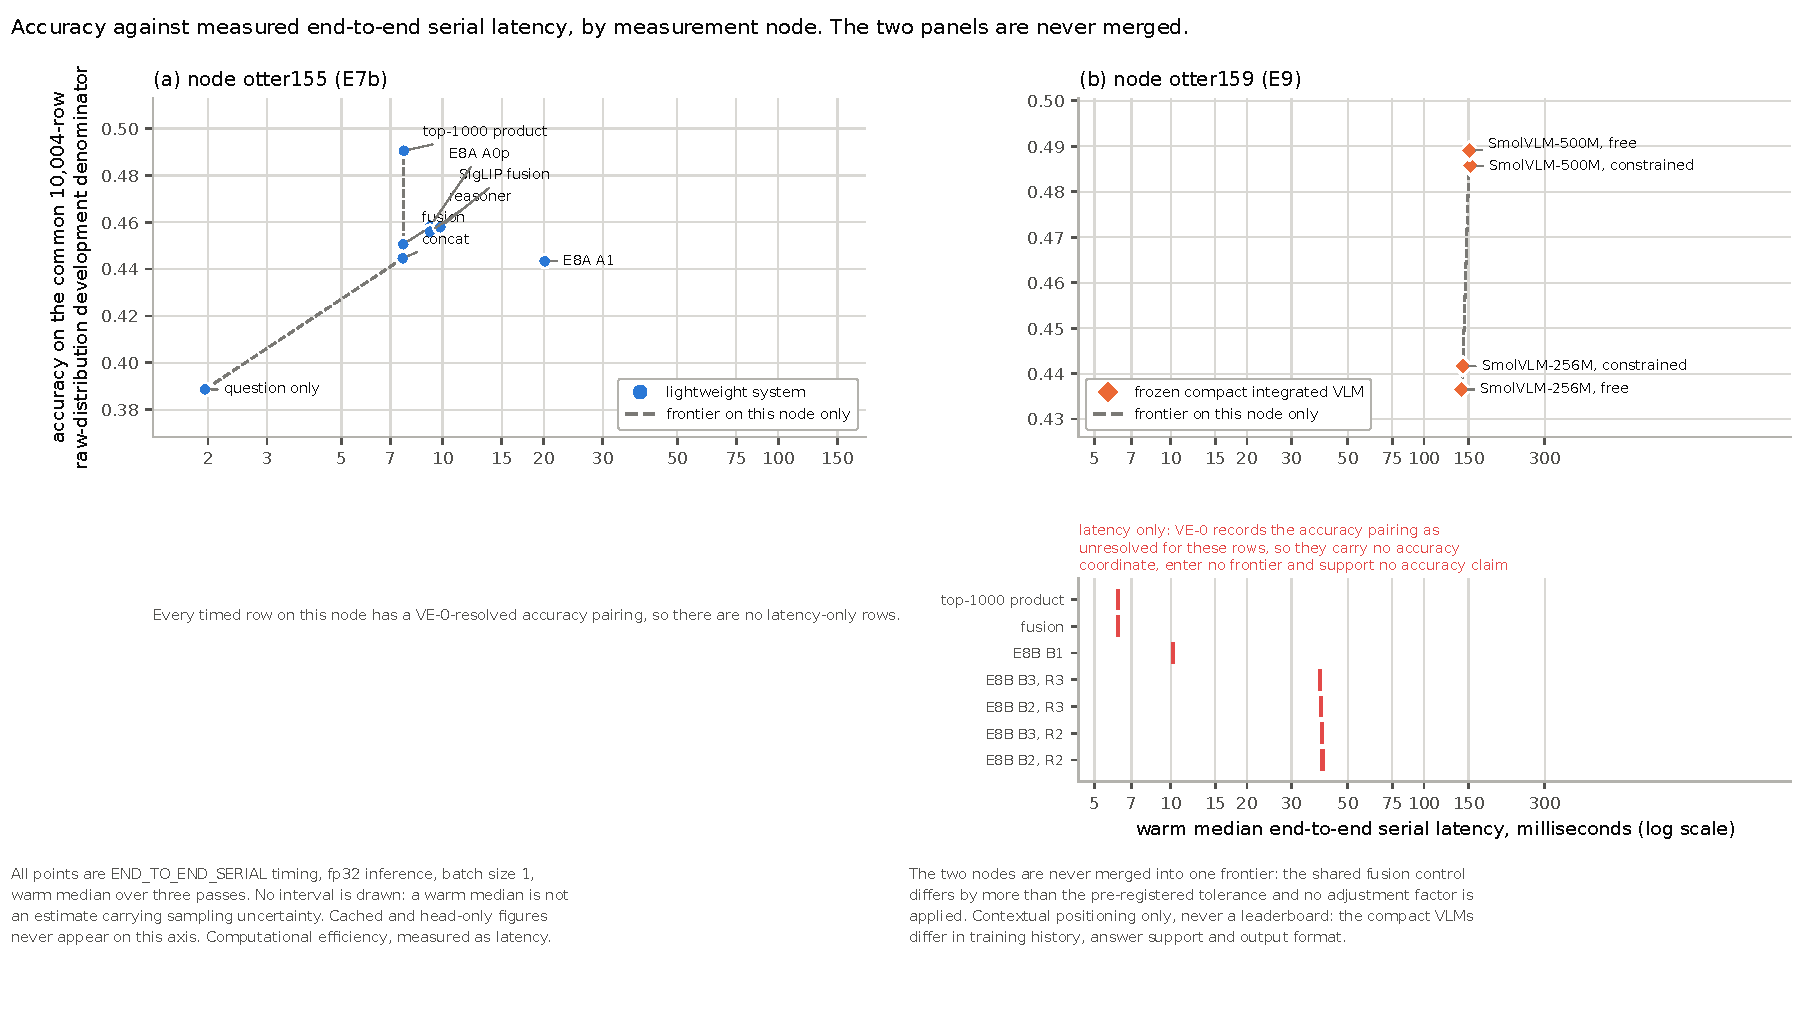
\includegraphics[width=0.98\textwidth]{images/ve1/VE1-FIG-09.pdf}
\caption[Accuracy against warm serial latency by node.]{Development accuracy against measured end-to-end warm serial latency, with \texttt{otter155} and \texttt{otter159} kept in separate panels. The fusion bridge differed by $-18.69\%$ against the $\pm10\%$ gate, so the nodes are never merged and no adjustment factor is used. Only end-to-end serial rows are shown: cached/head-only timings are not treated as end-to-end, and E7a additive sums are superseded. E9 is contextual and its unresolved reference rows are latency-only. E10 has no timing evidence. The figure supports computational latency claims only; it provides no energy, power, carbon or monetary-cost measurement.}
\label{fig:ch7-efficiency}
\end{figure}

\section{Parameter counts and interface cost}
\label{sec:ch7-parameters}

Table~\ref{tab:ch7-e7b} reports trainable parameter count separately from total
loaded parameter count. The former describes optimised capacity. The latter
counts parameters resident in the measured system under the E7b convention;
it is not checkpoint storage, file size, VRAM or a measured memory footprint.
Nominal labels such as 135M and 500M identify model families and should not be
read as trainable counts.

The global heads have between 576,100 and 1,624,676 trainable parameters in
the multimodal rows, while the latent reasoner, A0p and A1 have between
21,099,620 and 21,395,044. Their total loaded counts also differ because the
resident frozen towers differ. These counts establish capacity and residency
context, but they do not predict the observed latency ordering. No parameter
ratio is used as an efficiency result.

The answer-side timing boundary is narrower still. E9 times B1 and the B2/B3
R2 and R3 generation readouts on \texttt{otter159}. No serial latency was
measured for the Chapter-6 R1 likelihood readout, and R2/R3 timings are not its
cost. B4, B4r and E10 were not measured under a valid comparable headline
timing protocol. Parameter count alone is not used to fill these missing
measurements.

The retained segmented pass gives limited attribution context, while remaining
separate from the headline measurement. In that pass, the reasoner block takes
1.8014 ms, the SigLIP vision tower 4.9889 ms and the A1 SmolLM2 forward pass
13.4581 ms. These are segmented-pass components, not end-to-end latencies, and
they are not added to construct an alternative pipeline total. They describe
where time was observed within those instrumented passes without establishing
why one interface takes longer.

\section{Same-node compact-VLM context}
\label{sec:ch7-vlm}

Table~\ref{tab:ch7-e9} reports the E9 timing block on \texttt{otter159}, using
the imported serial harness with batch 1, 50 warm-up queries, 300 timed queries
and three passes. It is contextual evidence on a separate node, not an
extension of the E7b frontier. The re-timed top-1000 product head records
6.1990 ms under this timing protocol. The E9 artefact does not restate the
checkpoint identity for that row, so its accuracy is deliberately unavailable
in Table~\ref{tab:ch7-e9}.

Separately, the canonical development record gives the top-1000 product
system a common-view raw accuracy of 0.49050 on 10,004 rows. These facts are
not combined into a paired E9 coordinate. E9 does pair the SmolVLM rows with
their own G21 raw-distribution accuracies: the 256M
family records 0.436525 open and 0.441623 constrained, with latencies 140.9070
and 142.6747 ms; the 500M family records 0.489004 open and 0.485706
constrained, with latencies 151.3801 and 152.8540 ms.

The open rows use free greedy generation capped at 20 tokens. The constrained
rows use greedy decoding masked to the top-1000 answer-prefix trie. Both are
retained because they are paired E9 measurements, but the constrained readout
is a secondary diagnostic rather than a replacement accuracy protocol. The
B1 and B2/B3 rows in the same table are latency-only context: their missing
accuracy coordinates preserve the same unresolved-pairing boundary as the
re-timed head rows.

The canonical stored latency statement is that SmolVLM-500M constrained was
approximately 24.7 times slower in warm serial latency than the re-timed head
under the same-node contextual protocol. This statement compares latency only.
It does not create a paired accuracy comparison, a leaderboard or a general
claim about compact VLMs. The fusion bridge row is 6.2081 ms, but its failed
cross-node gate prevents any merge with the 7.6351 ms E7b fusion result.

\begin{table}[p]
\centering
\caption[E9 same-node timing context.]{Warm serial development timing on \texttt{otter159} under the E7b harness imported read-only. The block is contextual only: the fusion bridge failed, nodes are not merged, and no adjustment factor is used. Accuracy is shown only for the four canonically paired SmolVLM rows; re-timed product, fusion and B1/B2/B3 rows remain explicitly unpaired. No R1 answer-side latency exists, R2/R3 timings are not R1 cost, and E10 has no timing evidence.}
\label{tab:ch7-e9}
\begingroup\scriptsize\setlength{\tabcolsep}{0.65pt}
\makeatletter
\let\chSevenArrayParboxRestoreB\@arrayparboxrestore
\def\@arrayparboxrestore{\chSevenArrayParboxRestoreB\raggedright\let\\\tabularnewline}
\makeatother
\renewenvironment{longtable}[1]{\begin{tabular}{|p{0.14\textwidth}|p{0.15\textwidth}|p{0.10\textwidth}|p{0.115\textwidth}|p{0.085\textwidth}|p{0.07\textwidth}|p{0.10\textwidth}|p{0.07\textwidth}|}}{\end{tabular}}
\let\endhead\relax\renewcommand{\_}{\textunderscore\allowbreak}
% Generated by tools/tab2latex.py; do not edit.
% Presentation metadata: {"header_map":{"paired E9 raw accuracy":"Paired E9 raw accuracy","pairing status":"Pairing","role or readout":"Role or readout","spread ms":"Spread (ms)","system":"System","total loaded parameters":"Total loaded parameters","trainable parameters":"Trainable parameters","warm median ms":"Warm median (ms)"},"source_headers":["system","role or readout","trainable parameters","total loaded parameters","warm median ms","spread ms","paired E9 raw accuracy","pairing status"],"thousands":true}
\begin{longtable}{|l|l|l|l|l|l|l|l|}
\hline
System & Role or readout & Trainable parameters & Total loaded parameters & Warm median (ms) & Spread (ms) & Paired E9 raw accuracy & Pairing \\ \hline
\endhead
Top-1000 product & re-timed product head & 1,299,944 & 152,577,257 & 6.1990 & 0.0827 & unavailable & unpaired \\ \hline
Fusion bridge & cross-node bridge control & 1,100,388 & 152,377,701 & 6.2081 & 0.0179 & unavailable & unpaired \\ \hline
B1 classifier & LM-free classifier & 21,100,132 & 172,377,445 & 10.2420 & 0.4224 & unavailable & unpaired \\ \hline
B2 R2 & random 135M, constrained & 21,343,808 & 307,136,129 & 39.7326 & 1.4689 & unavailable & unpaired \\ \hline
B2 R3 & random 135M, open & 21,343,808 & 307,136,129 & 39.2394 & 1.2055 & unavailable & unpaired \\ \hline
B3 R2 & pretrained 135M, constrained & 21,343,808 & 307,136,129 & 39.6561 & 0.4844 & unavailable & unpaired \\ \hline
B3 R3 & pretrained 135M, open & 21,343,808 & 307,136,129 & 38.7963 & 0.3720 & unavailable & unpaired \\ \hline
SmolVLM-256M open & primary open generation & 0 & 256,484,928 & 140.9070 & 1.3031 & 0.436525 & resolved \\ \hline
SmolVLM-256M constrained & constrained diagnostic & 0 & 256,484,928 & 142.6747 & 0.7703 & 0.441623 & resolved \\ \hline
SmolVLM-500M open & primary open generation & 0 & 507,482,304 & 151.3801 & 1.2941 & 0.489004 & resolved \\ \hline
SmolVLM-500M constrained & constrained diagnostic & 0 & 507,482,304 & 152.8540 & 1.2409 & 0.485706 & resolved \\ \hline
\end{longtable}

\endgroup
\end{table}

% XREF-PENDING: appendix figure VE1-FIG-A5

\clearpage
\section{Efficiency summary}
\label{sec:ch7-summary}

Under the E7b protocol, the global multimodal heads occupy the lowest-latency
part of the governed multimodal set, at 7.6104--7.6708 ms, while the token-level
interfaces range from 9.1719 to 20.1460 ms. On the common 10,004-row
raw-distribution axis, concat, fusion and the top-1000 product head form the
canonical accuracy--latency frontier. The result is bounded to seed-0 250k
development checkpoints, otter155 and the stated serial measurement contract.

The E9 block gives separate same-node context for compact VLMs on otter159.
Its paired SmolVLM accuracies and latencies do not resolve the checkpoint
pairing of the re-timed product-head row, and the failed bridge prevents
cross-node merging. Accordingly, Chapter 7 supports claims about measured
warm serial latency, trainable parameter count and total loaded parameter
count only. Peak memory, storage size and environmental or monetary quantities
remain outside the retained evidence. No held-out inference follows from
these development measurements. Broader interpretation and design
implications are deferred to Chapter 8.
